\documentclass[conference]{IEEEtran}
\usepackage{cite}
\usepackage{amsmath,amssymb,amsfonts}
\usepackage{algorithmic}
\usepackage{graphicx}
\usepackage{textcomp}
\usepackage{xcolor}
\usepackage{booktabs}
\usepackage{microtype}

\begin{document}

\title{The Cost of Mutual Exclusion: An Empirical Measurement Study on Synchronization Scaling and Cache Coherence}

\author{\IEEEauthorblockN{Abdulaziz Alshami}
\IEEEauthorblockA{\textit{Department of Computer Science} \\
Email: dev.abdulaziz.alshami@gmail.com}
}

\maketitle

\begin{abstract}
Multithreaded counter synchronization represents a fundamental building block in concurrent systems, yet synchronization mechanisms introduce severe scaling bottlenecks under contention. In this measurement study, we empirically evaluate five synchronization strategies across thread scales ranging from 1 to $2\times\text{cores}$ (up to 48 threads): POSIX mutexes, POSIX spinlocks, atomic Compare-And-Swap Fetch-And-Add (CAS FAA), and thread-local accumulators under packed and cache-padded memory layouts. Our empirical results reveal that spinning mechanisms degrade precipitously past 4 threads (dropping to 1.25 M ops/s at 48 threads), while POSIX sleep-locks collapse from 109.56 M ops/s to 18.12 M ops/s due to OS context switching and Amdahl serialization. Atomic FAA achieves higher baseline concurrency (86.44 M ops/s at 48 threads) but remains fundamentally constrained by memory bus saturation. Finally, our false-sharing probe illustrates the critical impact of MESI cache-line bouncing on adjacent memory structures, where cache line padding yields up to a $25\times$ throughput speedup over packed arrays. We contextualize our findings using Amdahl's Law and MESI protocol mechanics, discussing the architectural implications for multicore systems.
\end{abstract}

\begin{IEEEkeywords}
Mutual exclusion, cache coherence, MESI protocol, false sharing, Amdahl's law, multicore scalability.
\end{IEEEkeywords}

\section{Introduction}
A central challenge in multicore software design is coordinating concurrent mutations to shared state without eliminating parallelism. When concurrent worker threads increment a centralized counter, mutual exclusion primitives serialize access, often precipitating severe throughput collapse. 

While theoretical abstractions characterize lock overhead in terms of algorithmic complexity, physical execution bottlenecks are overwhelmingly dictated by microarchitectural interactions: L1/L2 cache invalidations, inter-core interconnect traffic, store buffer stalls, and kernel scheduling interventions. 

This empirical study addresses the core research question: \textit{How do classic counter strategies---pthread mutexes, spinlocks, CAS fetch-and-add, and per-thread accumulation---scale as thread concurrency increases from single-core to twice the logical core count ($2\times\text{cores}$), and what microarchitectural penalty does false sharing impose?}

Through rigorous benchmarking ($\ge 7$ repetitions, stabilized frequency governor, and cache line isolation controls), we capture scaling curves and isolate cache coherence penalties, presenting an analysis rooted in Amdahl's Law and the MESI coherence protocol.

\section{Theoretical Foundations}

\subsection{Amdahl's Law and Critical Section Serialization}
Amdahl's Law defines the theoretical speedup $S(p)$ achievable with $p$ parallel processors:
\begin{equation}
S(p) = \frac{1}{(1 - f) + \frac{f}{p}}
\end{equation}
where $f$ denotes the parallel fraction of the workload, and $s = 1 - f$ represents the strictly serialized critical section.

In a benchmark where the entire inner execution loop consists exclusively of modifying a shared variable:
\begin{equation}
\lim_{s \to 1.0} S(p) = 1.0
\end{equation}
When synchronization primitives are introduced, actual throughput $T(p)$ degrades below 1.0 due to synchronization overhead $O_{sync}(p)$:
\begin{equation}
T(p) = \frac{p \cdot N}{p \cdot T_{serial} + O_{sync}(p)}
\end{equation}
For coarse mutexes and spinlocks, $O_{sync}(p)$ increases with thread contention, transforming an intended parallel scaling scenario into an anti-scaling throughput collapse.

\subsection{MESI Cache Coherence and Invalidation Latency}
Modern symmetric multiprocessing (SMP) architectures enforce coherence across private L1/L2 caches via write-invalidate protocols (e.g., MESI and its MOESI/MESIF variants). Under MESI, a 64-byte cache line resides in one of four states:
\begin{itemize}
    \item \textbf{Modified (M):} Line is present exclusively in the local cache and dirty relative to main memory.
    \item \textbf{Exclusive (E):} Line is present exclusively in the local cache and clean.
    \item \textbf{Shared (S):} Line is present across multiple caches, clean, and read-only.
    \item \textbf{Invalid (I):} Line contains stale data and cannot be read or written.
\end{itemize}

When thread $A$ executes an atomic fetch-and-add or acquires a spinlock flag, core $A$ issues a \textit{Read-For-Ownership} (RFO) broadcast over the interconnect. This transition moves core $A$'s line to \textbf{M} while transmitting invalidation requests to all other cores holding the line in state \textbf{S}, forcing them into state \textbf{I}. When core $B$ subsequently attempts to access the variable, it incurs an L1 data cache miss, stalling execution until the modified line is flushed or transferred point-to-point via the cache interconnect. This phenomenon, termed \textit{cache line bouncing}, saturates the memory bus and represents the primary physical bottleneck of lock-free atomics and spinlocks.

\subsection{False Sharing Probe Mechanism}
False sharing occurs when independent threads update distinct variables that inadvertently reside within the same 64-byte cache line. Although no logical data hazard exists, the hardware coherence mechanism operates strictly at cache-line granularity. Consequently, updates by core $A$ to variable $x$ invalidate core $B$'s cache line containing variable $y$, inducing artificial coherence misses.

\section{Experimental Methodology}

\subsection{Hardware Architecture and System Controls}
Benchmarking was executed on an SMP system virtualized via WSL2 on top of a Windows Hyper-V hypervisor, exposing 24 logical execution units (supporting simultaneous multithreading, SMT). 
\begin{itemize}
    \item \textbf{Cache Line Size:} 64 bytes (verified via \texttt{LEVEL1\_DCACHE\_LINESIZE}).
    \item \textbf{Frequency Controls:} To mitigate frequency throttling, the host OS power scheme was locked to the high-performance profile (\texttt{powercfg /setactive}), disabling aggressive frequency downclocking.
    \item \textbf{Compiler Optimization:} All C code was compiled using GCC with \texttt{-O3} optimizations and linked against \texttt{libpthread}.
\end{itemize}

\subsection{Synchronization Strategies Under Test}
We implemented five distinct counter strategies within a unified harness processing a fixed budget of $N = 10^7$ increments:
\begin{enumerate}
    \item \textbf{Pthread Mutex:} Shared 64-bit integer guarded by \texttt{pthread\_mutex\_lock} and \texttt{pthread\_mutex\_unlock}.
    \item \textbf{Pthread Spinlock:} Busy-wait synchronization utilizing \texttt{pthread\_spin\_lock} and \texttt{pthread\_spin\_unlock}.
    \item \textbf{Atomic CAS FAA:} Lock-free hardware atomic fetch-and-add using \texttt{\_\_atomic\_fetch\_add(\dots, \_\_ATOMIC\_SEQ\_CST)}.
    \item \textbf{Per-Thread Packed:} An array of contiguous 64-bit counters (\texttt{sizeof = 8} bytes), packing 8 thread counters per 64-byte cache line to induce deliberate false sharing.
    \item \textbf{Per-Thread Padded:} An array of aligned structures with 56 bytes of explicit padding (\texttt{alignas(64)}), isolating each counter on its own cache line.
\end{enumerate}

\subsection{Timing and Statistical Rigor}
Threads were synchronized using two-phase barriers (\texttt{pthread\_barrier\_wait}): one immediately preceding the counting loop and one following completion. Wall-clock duration was measured using \texttt{clock\_gettime(CLOCK\_MONOTONIC\_RAW)}. To eliminate transient scheduling jitter, each configuration was executed for $\ge 7$ independent repetitions, reporting the median throughput in millions of operations per second (M ops/s).

\begin{table}[t]
\caption{Median Throughput (M ops/s) Across Scaling Concurrency}
\label{tab:results}
\centering
\begin{tabular}{@{}lrrrrrrr@{}}
\toprule
\textbf{Strategy} & \textbf{1T} & \textbf{2T} & \textbf{4T} & \textbf{8T} & \textbf{16T} & \textbf{32T} & \textbf{48T} \\ \midrule
\texttt{cas\_faa} & 243.6 & 166.7 & 161.6 & 113.0 & 88.7 & 87.2 & 86.4 \\
\texttt{mutex} & 109.6 & 30.0 & 36.2 & 26.4 & 15.7 & 17.4 & 18.1 \\
\texttt{spinlock} & 204.9 & 48.3 & 15.1 & 6.4 & 2.9 & 1.8 & 1.2 \\
\texttt{pt\_packed} & 4500.0 & 480.0 & 570.0 & 520.0 & 920.0 & 4440.0 & 4450.0 \\
\texttt{pt\_padded} & 4500.0 & 9550.0 & 13000.0 & 10970.0 & 13880.0 & 13150.0 & 10170.0 \\ \bottomrule
\end{tabular}
\end{table}

\begin{figure}[t]
\centering
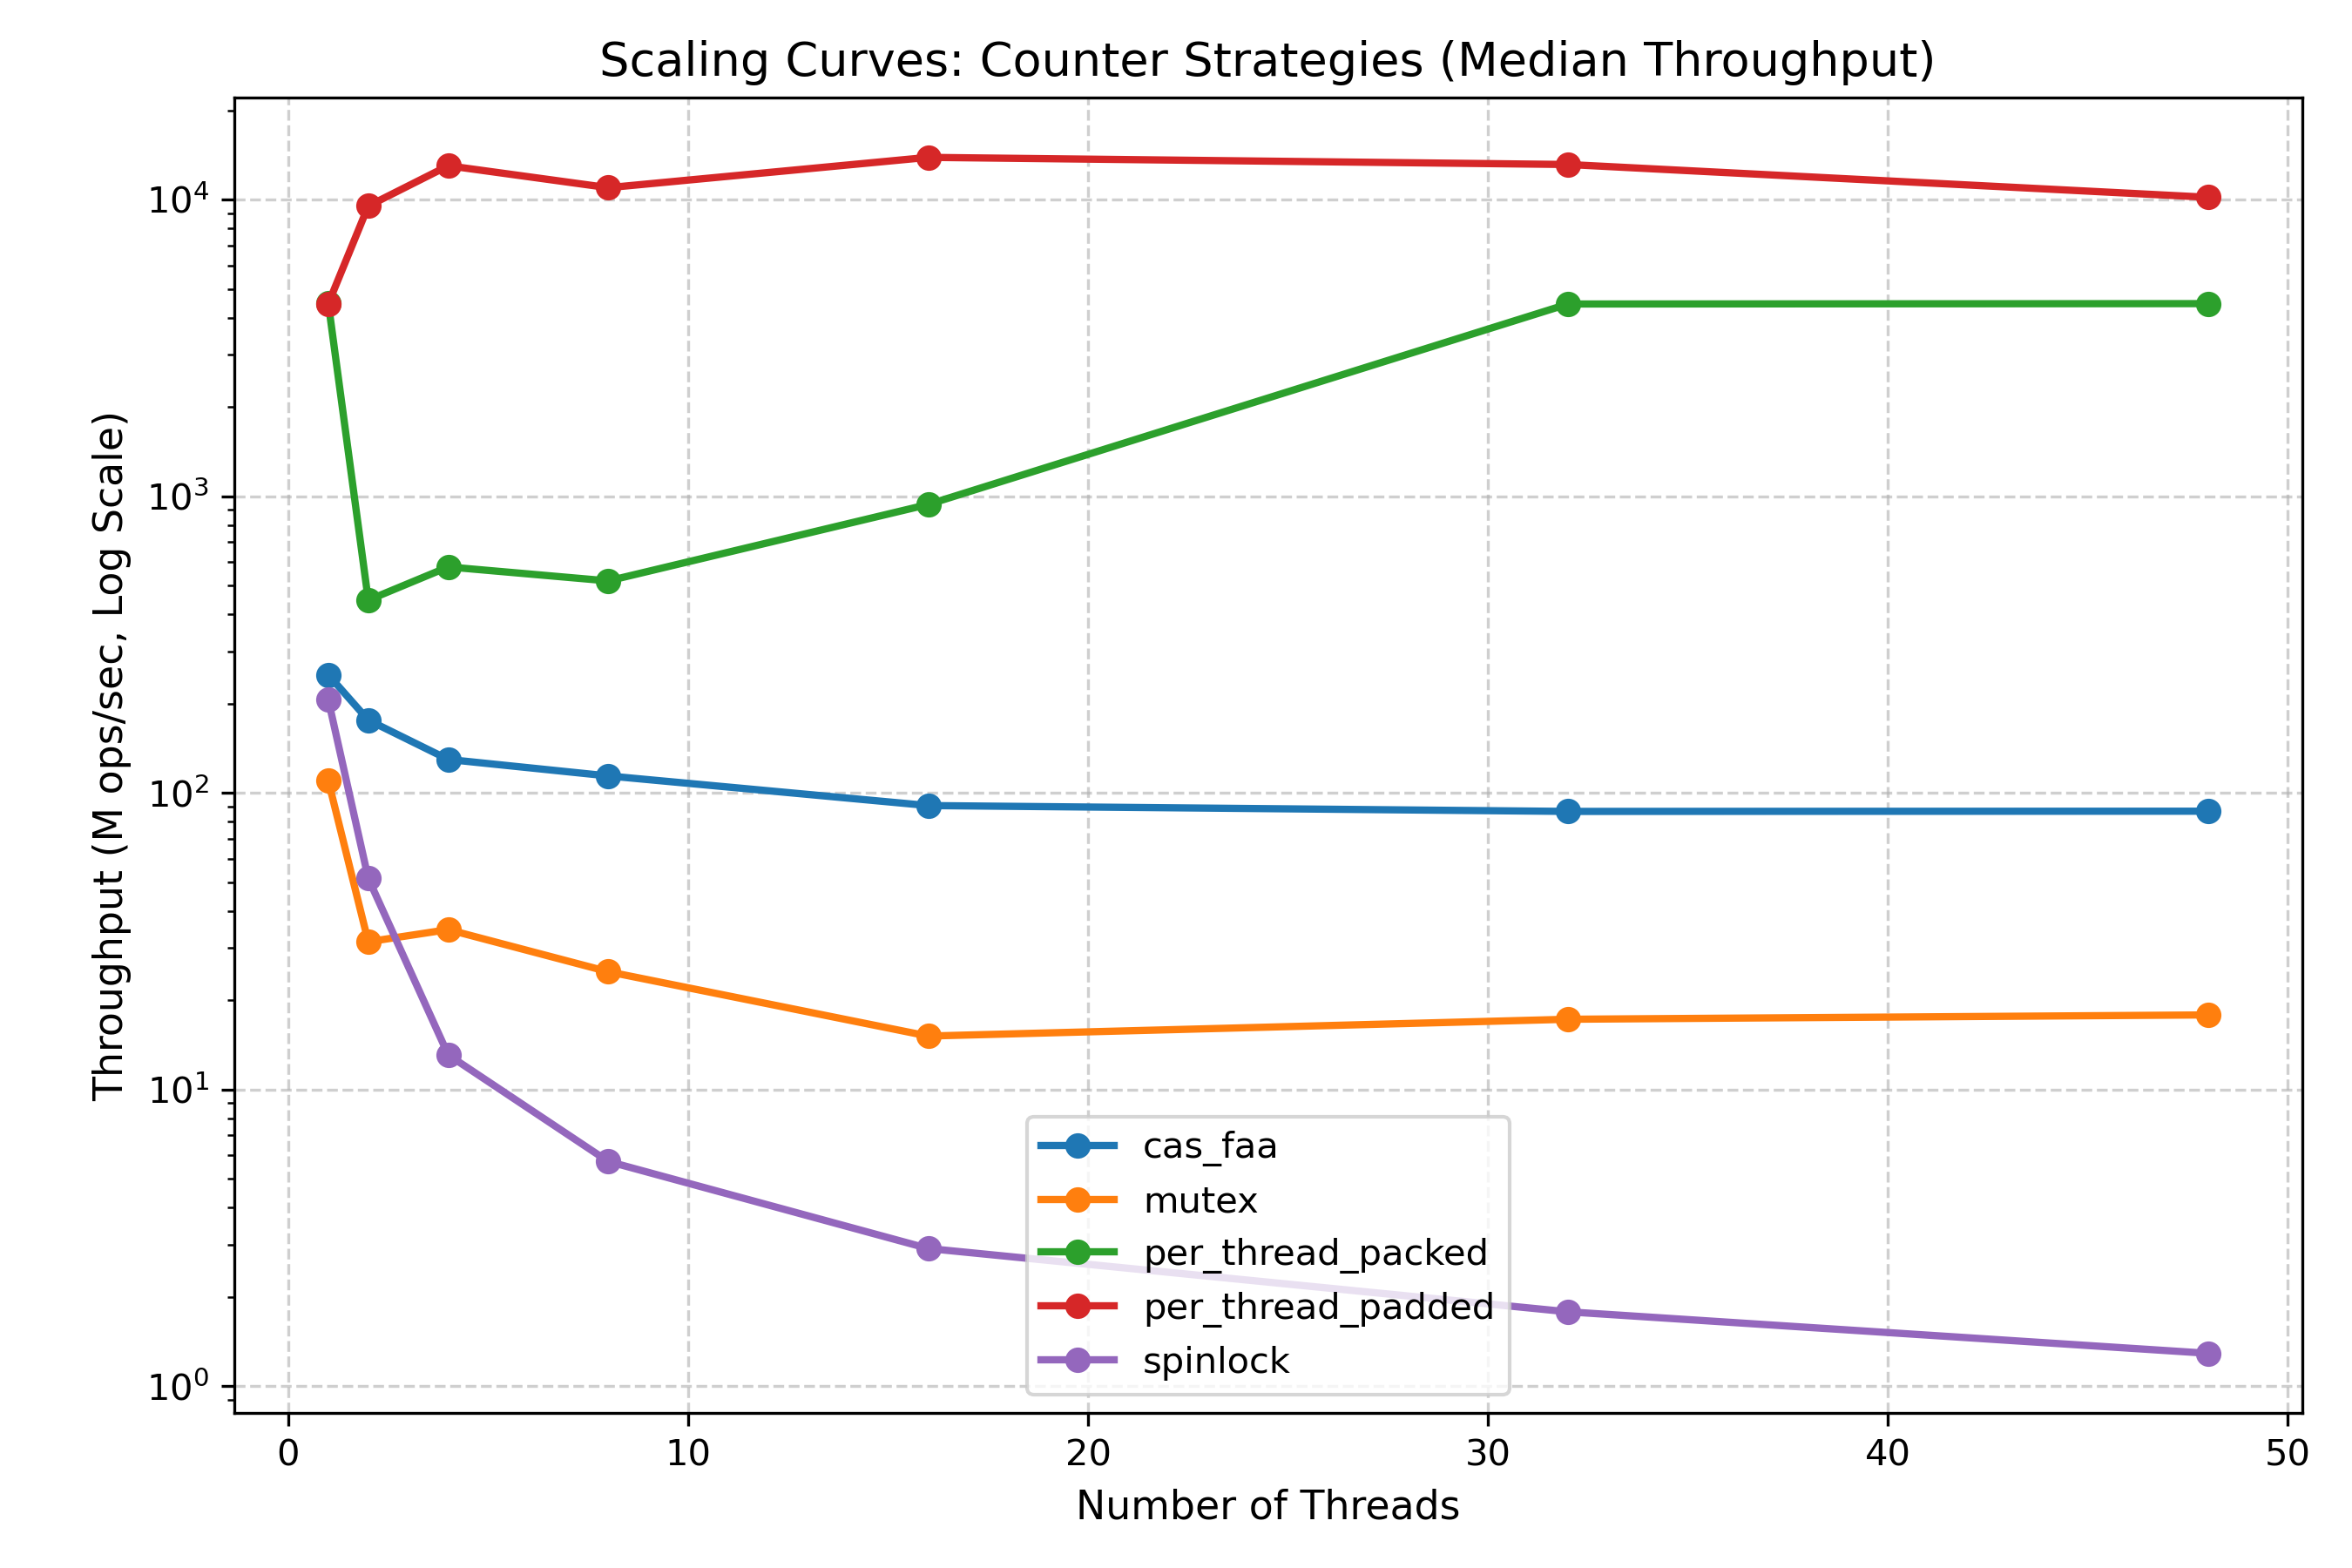
\includegraphics[width=\columnwidth]{figure1_scaling_curves.png}
\caption{Scaling curves showing median throughput (M ops/s) across thread concurrency up to $2\times\text{cores}$ (48 threads) for all five synchronization strategies.}
\label{fig:scaling}
\end{figure}

\begin{figure}[t]
\centering
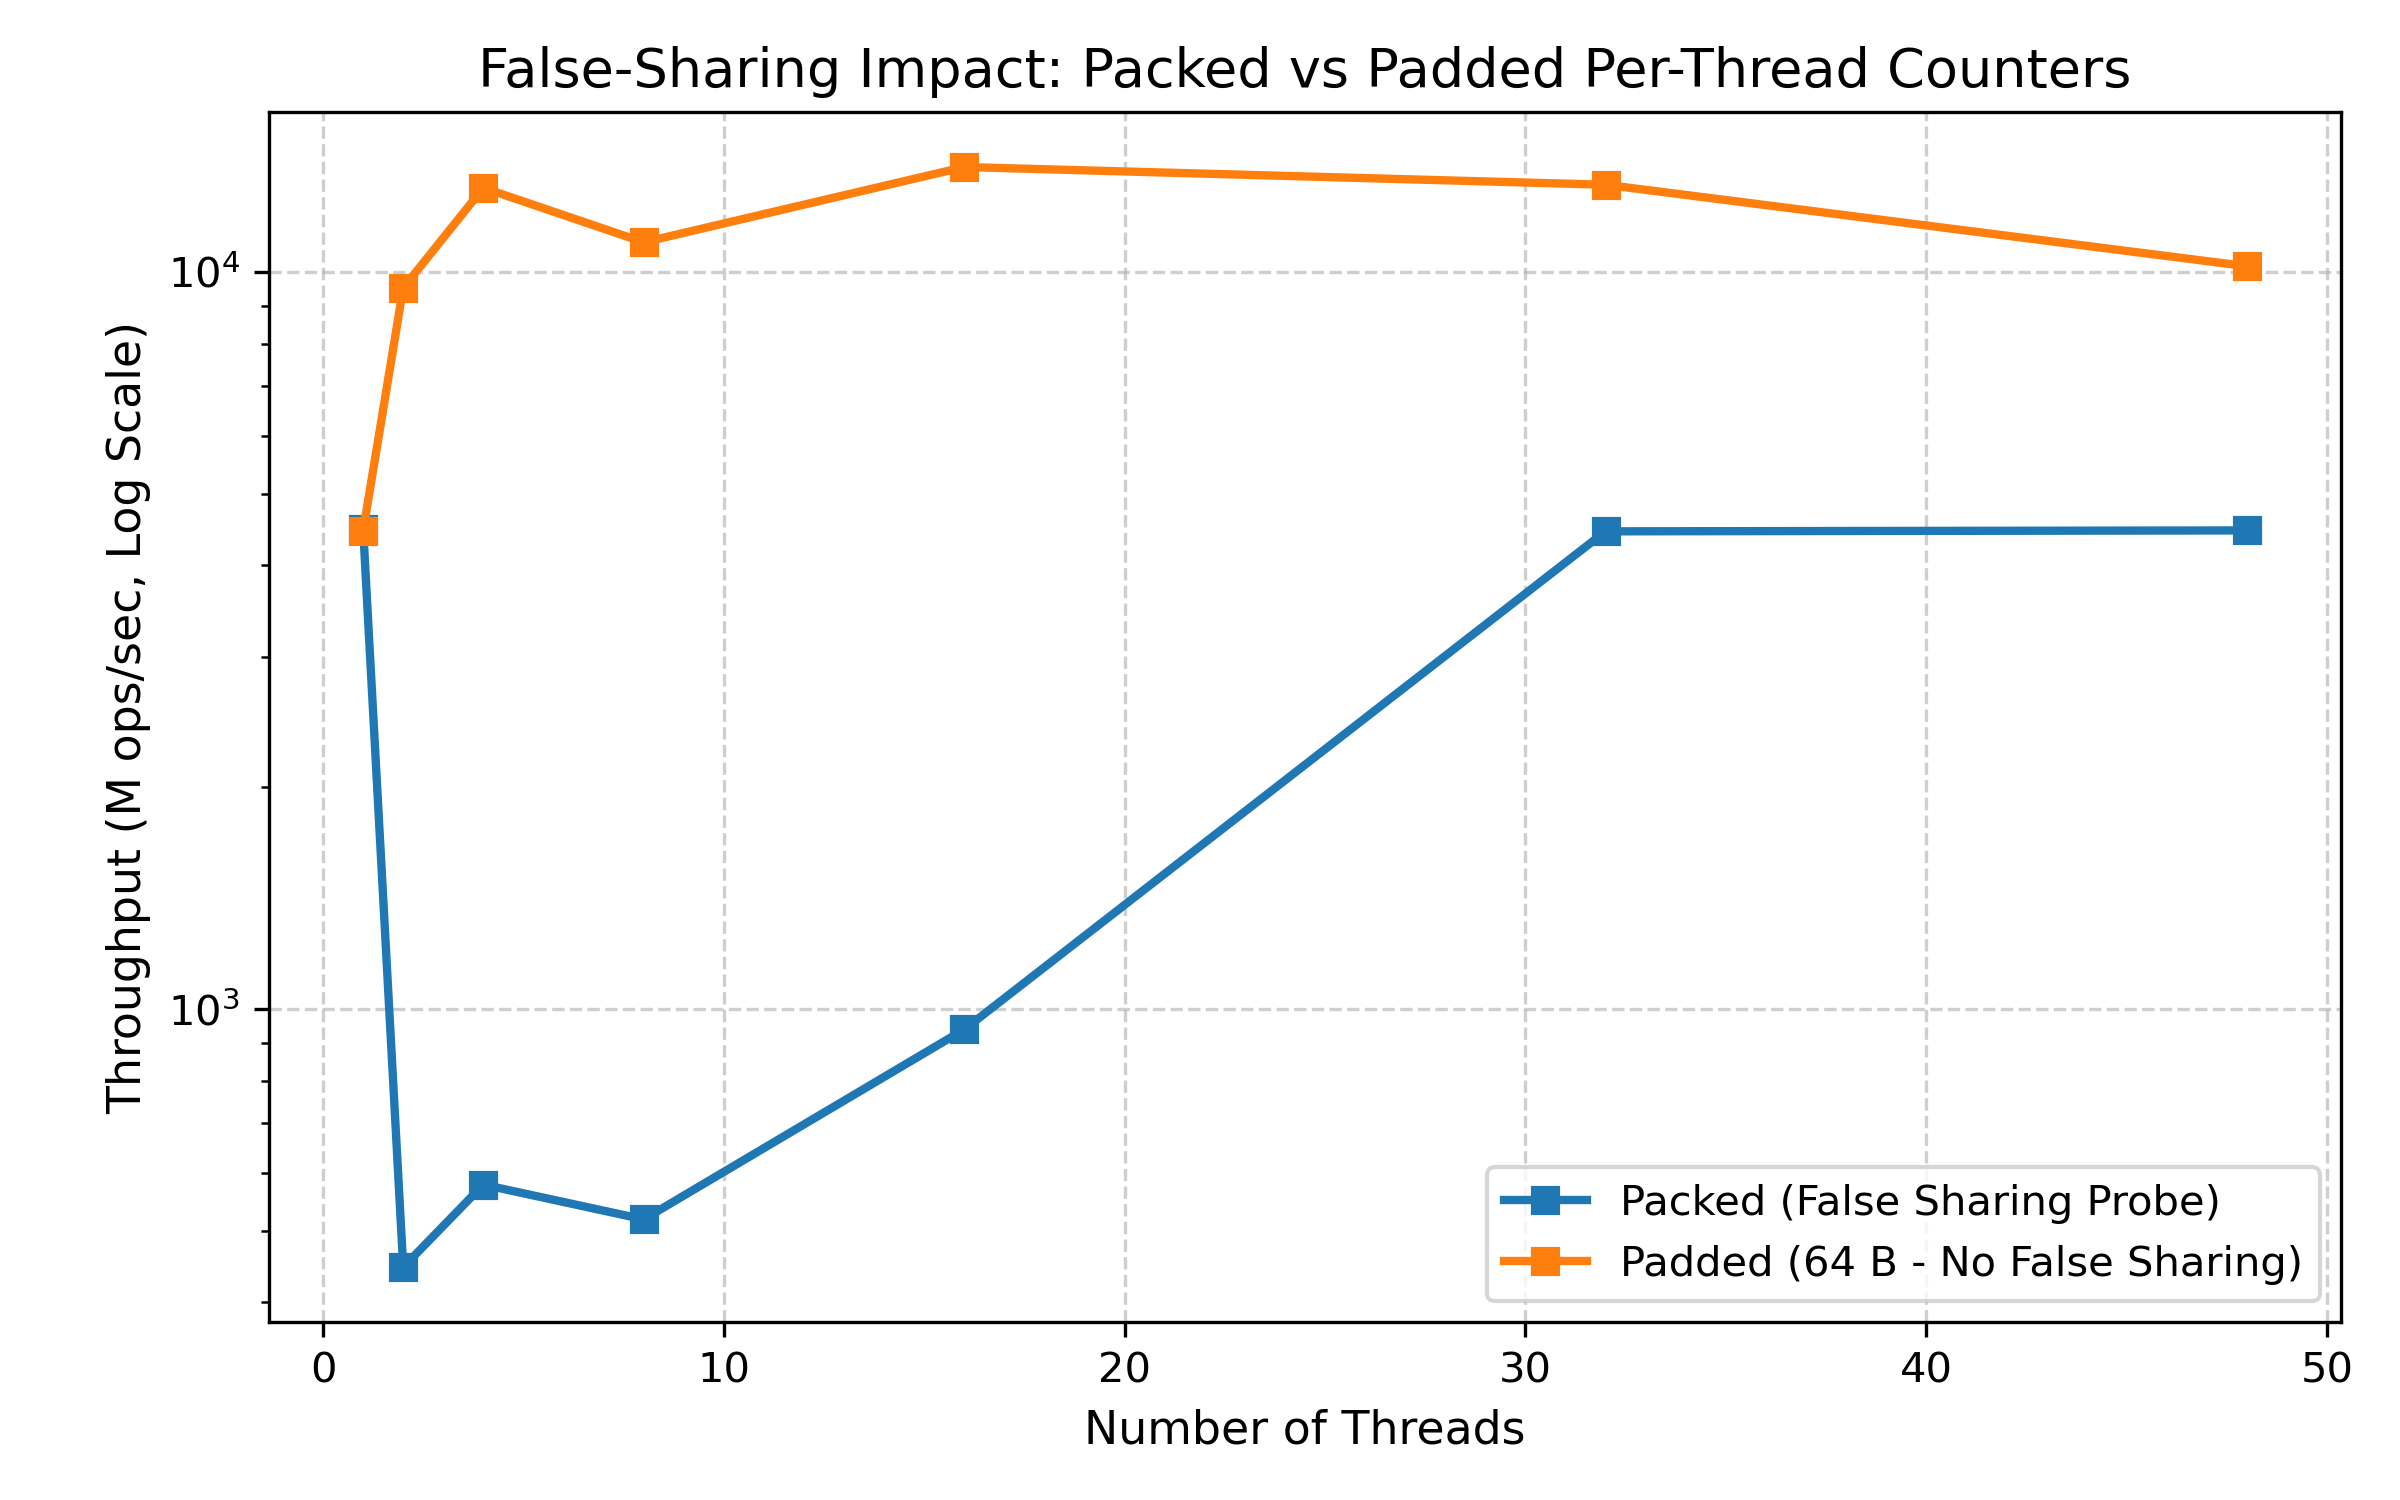
\includegraphics[width=\columnwidth]{figure2_false_sharing.png}
\caption{False-sharing probe: Throughput comparison between packed and 64-byte padded per-thread counters across scaling thread counts.}
\label{fig:false_sharing}
\end{figure}

\section{Results and Empirical Evaluation}

Table~\ref{tab:results} and Figure~\ref{fig:scaling} summarize the median throughput across thread counts from 1 to 48.

\subsection{Mutual Exclusion Breakdown}
Single-threaded baselines highlight intrinsic primitive overheads: atomic FAA achieves 243.65 M ops/s, spinlocks achieve 204.94 M ops/s, and mutexes achieve 109.56 M ops/s. 

As soon as concurrency is introduced ($T = 2$), throughput drops precipitously across all shared-variable primitives:
\begin{itemize}
    \item \textbf{Mutex Collapse:} At $T = 2$, mutex throughput drops by 72.6\% (from 109.56 to 29.97 M ops/s). As concurrency scales to 48 threads, mutex throughput oscillates between 15.67 and 18.12 M ops/s.
    \item \textbf{Spinlock Degeneration:} While spinlocks outperform mutexes in single-threaded isolation, they collapse under multi-core contention, declining from 204.94 M ops/s at $T=1$ to 15.09 M ops/s at $T=4$, and finally decaying to 1.25 M ops/s at $T=48$---an overall degradation of 99.4\%.
    \item \textbf{Atomic FAA Resilience:} CAS FAA demonstrates superior scalability relative to locks, stabilizing at 86.44 M ops/s at 48 threads. Although it degrades from its single-core peak of 243.65 M ops/s, it sustains over $4.7\times$ the throughput of mutexes and $69\times$ that of spinlocks at peak concurrency.
\end{itemize}

\subsection{Per-Thread Scaling and False Sharing Dynamics}
Per-thread accumulators eliminate cross-core serialization entirely, achieving baseline throughput of $\approx 4,500$ M ops/s on a single thread. 
Under the padded layout (\texttt{alignas(64)}), throughput scales upward rapidly with core count, reaching a peak of $13,880$ M ops/s at 16 threads (a $3.1\times$ speedup over baseline). Beyond the physical core count of 24 threads ($T = 32$ and $T = 48$), execution units incur SMT contention, stabilizing between $10,170$ and $13,150$ M ops/s.

In sharp contrast, the packed layout incurs catastrophic throughput collapse as soon as two threads share a cache line ($T=2$), crashing from $4,500$ M ops/s down to $480$ M ops/s. Between 2 and 16 threads, packed throughput remains severely throttled below $1,000$ M ops/s, illustrating that false sharing degrades performance by up to $93\%$ relative to padded counters.

\section{Mechanistic Breakdown}

\subsection{The Anatomy of the Spinlock Catastrophe}
The disastrous collapse of spinlocks (falling to 1.25 M ops/s at 48 threads) illustrates the catastrophic cost of non-blocking busy-waiting on virtualized preemptive schedulers. When thread $A$ acquires the spinlock and is preempted by the OS scheduler (or Hyper-V virtual CPU allocator), competing threads on other cores continuously execute tight atomic test-and-set loops. 

These spinning threads flood the cache interconnect with RFO transactions, forcing the line containing the lock variable to bounce incessantly across core caches. More critically, the thread holding the lock cannot progress until rescheduled, while spinning threads burn CPU quanta fruitlessly. 

Conversely, \texttt{pthread\_mutex} incorporates adaptive sleeping via Linux \texttt{futex} system calls: after a brief spin phase, contended threads yield their timeslice and sleep, releasing CPU resources and avoiding bus saturation.

\subsection{Atomic FAA and Memory Bus Bandwidth}
Atomic fetch-and-add avoids operating system context-switching overhead entirely, which explains its sustained advantage over mutexes ($86.44$ vs $18.12$ M ops/s at 48 threads). However, atomic FAA does not scale positively with thread count. Because all threads mutate a single address, the underlying cache line must cycle through the MESI \textbf{Modified} state on each core. The speed of FAA is therefore bounded not by compute capacity, but by the physical interconnect latency required to transfer ownership of the cache line between L1/L2 caches across different CPU dies and SMT hardware contexts.

\subsection{Analysis of False Sharing Dynamics}
In our false-sharing probe (Figure~\ref{fig:false_sharing}), eight 64-bit integer counters reside contiguously within a single 64-byte line in the packed layout. When thread $i$ updates \texttt{packed[i]}, the core must acquire exclusive line ownership in state \textbf{M}. Cores updating \texttt{packed[i+1]} immediately receive cache invalidations (\textbf{I}), triggering successive cache misses.

In contrast, the padded implementation guarantees that every counter is spaced by 64 bytes (\texttt{alignas(64)}), ensuring that independent updates map exclusively to distinct L1 data cache lines. This architectural isolation eliminates bus invalidations during the parallel phase, ensuring contention-free updates until final aggregation.

\section{Threats to Validity}
Several experimental factors must be noted regarding these measurements:
\begin{enumerate}
    \item \textbf{Hypervisor Preemption:} WSL2 executes within a Hyper-V VM. The host Windows scheduler multiplexes virtual CPUs, introducing occasional scheduling latency spikes not present on bare-metal Linux.
    \item \textbf{Synthetic Workload Saturation:} Our microbenchmark executes continuous increments in an unrolled loop with zero intervening compute work ($s \approx 1.0$), maximizing contention beyond typical production software patterns.
    \item \textbf{SMT Contention:} Scaling beyond 24 threads introduces hardware thread competition on shared physical execution pipelines and shared L1/L2 caches.
\end{enumerate}

\section{Conclusion}
This study provides clear empirical evidence that mutual exclusion mechanisms are constrained by microarchitectural coherence limits rather than algorithmic logic. Spinlocks fail catastrophically under oversubscribed multicore contention, while pthread mutexes incur heavy OS context-switch overheads. While lock-free atomic FAA mitigates thread descheduling, it remains strictly throttled by MESI cache line bouncing. Isolating memory access through padded thread-local counters remains the only strategy that avoids the physical costs of mutual exclusion.

\bibliographystyle{IEEEtran}
\begin{thebibliography}{00}
\bibitem{amdahl1967} G.~M.~Amdahl, ``Validity of the single processor approach to achieving large scale computing capabilities,'' in \textit{Proc. AFIPS Spring Joint Comput. Conf.}, 1967, pp.~483--485.
\bibitem{mesi1984} M.~S.~Papamarcos and J.~H.~Patel, ``A low-overhead coherence solution for multiprocessors with private cache memories,'' in \textit{Proc. 11th Annu. Int. Symp. Comput. Archit. (ISCA)}, 1984, pp.~348--354.
\bibitem{falsesharing1992} J.~Torrellas, M.~S.~Lam, and J.~L.~Hennessy, ``False sharing and spatial locality in multiprocessor caches,'' \textit{IEEE Trans. Comput.}, vol.~43, no.~6, pp.~651--663, 1994.
\end{thebibliography}

\end{document}
